\section{Framework}
We have developed a software framework, Senseless, which provides a common data interface to the WSNs and GUIs. It also controls the data flows between the WSNs and GUIs, and stores this data in a database for later retrieval. The system is capable of working with different algorithms and new algorithms can be easeliy added. If there are three anchor nodes available, we can work with range-based algorithms, thus obtaining a better accuracy. If, on the other hand, only one anchor node is available, a connectivity-based algorithm can and must be used. We will use this system to test the different localization algorithms and analyze the RSS data. 

Senseless has a Model-View-Controller (MVC) design, as in Figure \ref{fig:mvc}; the system is divided into three different parts each with different tasks. The separation of these responsibilities enhances the modularity of the system. 
The details of this design are as follows:
\begin{itemize}
	\item Model: This layer defines the representation of the information which the application works with. The data is stored in a MySQL database. 
	\item View: Information can be accessed and controlled via this part. User interfaces are defined in this layer. The view does not process data. 
	\item Controller: It processes and uses polling to react to events, mostly caused by the actions of the user and the data delivered by the WSN. 
\end{itemize}
The advantage of this design pattern is that we can easily add views and models without changing the whole system. 

\begin{figure}[h]
	\centering
		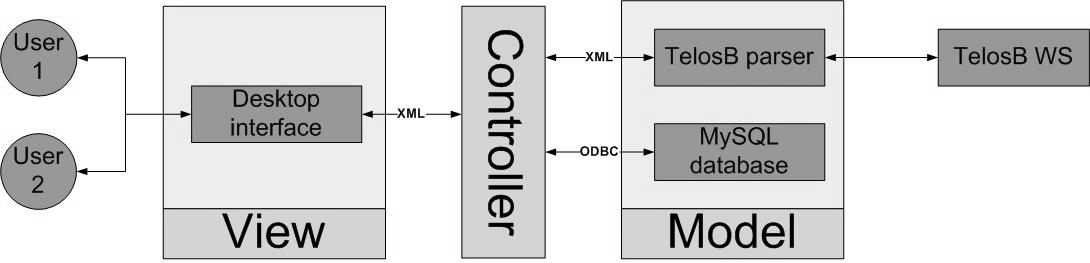
\includegraphics[scale=0.30]{Images/mvc.jpg}
	\caption{The Model-View-Controller design}
	\label{fig:mvc}
\end{figure}

\subsection{Functionality}
The system consists of four main parts:
\begin{itemize}
	\item WSN
	\item Database
	\item Graphical Unit Interface (GUI)
	\item Controller
\end{itemize}

\subsubsection{WSN}
The WSN consists of Telos rev.B nodes, which have the following specifications: 
\begin{itemize}
	\item TI MSP430 microcontroller with 10kB RAM 
	\item IEEE 802.15.4 compliant CC2420 radio: it supports eight discrete power levels and 16 channels
	\item Integrated temperature, light, humidity and voltage sensor 
	\item TinyOS 2.X compatible 
	\item Programmable via USB interface 
	\item Integrated antenna 
\end{itemize}

Each node fulfills one of the three different roles: 
\begin{itemize}
	\item Root node (RN): this node receives data from the rest of the network , and acts as a bridge between the WSN and the rest of the framework. The root sends these messages to the controller via an XML parser. It also receives commands from the controller and disseminates these to the right node.
	\item Anchor node (AN): this node has a known location, and broadcasts a message with its ID to the blind nodes and anchor nodes for calibration. The node also transmits its sensor data to the root with the sensor message. 
	\item Blind node (BN): this node has an unknown location and receives broadcast messages from the anchor nodes. The node uses these messages to determine the RSS, and transmits the RSS together with the ID of the anchor node to the root with the location message. The blind node also transmits its sensor data to the root node with the sensor message. 
\end{itemize}

There are three different data messages which are collected from the wireless network:
\begin{itemize}
	\item	Sensor messages, which contain the data collected by the sensors of the nodes.
	\item Location messages, which contain data relevant to locate the blind node.
	\item Status messages, which contain data that represent the status of the node transmitting the message.
\end{itemize}

\subsubsection{Database}
We implemented a MySQL 5.0 database to store the data generated by the system, but any ODBC-compliant database can be used.  

\subsubsection{GUI}
The user interfaces provides us with the ability to easily control and monitor the WSN. Rapid deployment was the key motivator to build this component. Using this, the user can set several node parameters, with a focus on localization: sampling period, coordinates (in meters), inactive/active, blind/anchor and the leds. This can be done in a few seconds. In contrast to manually hardcoding every single node of the network, which can be very time-consuming and sometimes impossible due to the fact that TinyOS-programmed nodes and other types of nodes usually provide very little to no user interaction. 

\subsubsection{Controller}
The controller is the core of our system. The controller is programmed in C# using the .NET 3.5 framework.  It is divided into several class library's and a single Windows Forms project.

It has four main functions:

Firstly, the controller acts as a gatekeeper to the database, ensuring that all data is stored in the correct table and is of the correct type. This is especially important for WSNs as a plethora of hardware platforms exist. These platforms have different data types and can have a different endianness.

Secondly, the controller is also a central gathering point for all the data. By using the controller in our framework, every other component can use a single data interface and should only be aware of the location of the controller.

Thirdly, an interface to Scala is provided as well. Scala is a middleware for location systems. Scala and the interface will be described in the designated section.
Finally, the controller implements the centralized versions of our localization algorithms. The user can instruct the controller to use an algorithm via a simple Windows Forms GUI.

\textbf{WSN vs Controller}

The communication between the WSN and the controller is done with an XML parser, which translates the messages of both sides into XML and back into an internal format. The root node of the WSN receives all the messages (sensor, location and status) from the nodes and forwards these to the controller, or if the controller needs to pass a command on to the root, it will be forwarded to the root. With the help of the dissemination protocol, the command is transmitted over the WSN. 

\textbf{Controller vs GUI}

The communication between the controller and the GUI also happens with an XML parser, which translates the messages that need to be exchanged. Firstly, the GUI displays the data from the WSN, thus a request needs to be send to the controller. The controller receives the request, and gets the data out of the database and sends it to the GUI. Secondly, the GUI is used to control the WSN. If, for example, you want to change the sample rate of the WSN, then a command will be sent to the controller which forwards it to the root node of the WSN. 

\textbf{Controller vs Database}

The communication here makes use of ODBC (Open Database Connectivity), which is an universal database interface. By using this interface, the controller does not need to worry about the database that is used. Stored procedures are used instead of full SQL syntax.

\subsection{SCALA}
SCALA is a TETRA \cite{tetra} project which aims to shorten the gap between localization technologies and possible end-user applications. The goal of this project is to ease the development of location aware applications by providing these applications with a common interface to the location technologies.

From a technical point of view, SCALA adapts the interfaces of the existing localization technologies into a common interface. Doing so, the user can receive location information transparent of the underlying technology. 
Another feature of SCALA is the fusion of location information. By combining the information the middleware receives from different localization technologies, a more accurate and robust position can be determined.

The Senseless framework will provide an interface to SCALA. The framework will plug into SCALA as an engine. Doing so, our algorithms become accessible to a variety of applications.
The interface with the middleware is constructed in the controller. Two types of communication are available: polling and event-based. By polling the engine, information is requested only when needed, as opposed to event-based communication where, the middleware subscribes to information coming from the WSN. The interface is loosely based on the ANSI Rtls API \cite{RTLS}.
The API documents a polling-based system. Possible data fields are specified and a method of filtering data is documented as well.
